%author: Mouad Jaouhari
%version : 1
%date : 17 June 2025

\documentclass[a4paper,12pt]{extarticle} % Classe du document

%--------------------- Packages ------------------------

\usepackage[french]{babel} %Langue du document
\usepackage[utf8]{inputenc} %Caractères spéciaux
\usepackage[section]{placeins}%Pour placement de section
\usepackage[T1]{fontenc} %Quelques lettres qui sont pas inclus dans UTF-8
\usepackage{mathtools} %Paquet pour des équations et symboles mathématiques
\usepackage{siunitx} %Pour écrire avec la notation scientifique (Ex.: \num{2e+9})
\usepackage{float} %Pour placement d'images
\usepackage{graphicx} %Paquet pour insérer des images
\usepackage[justification=centering]{caption} %Pour les légendes centralisées
\usepackage{subcaption}
\usepackage{wallpaper}
\usepackage{nomencl}
\usepackage{amsmath}
\usepackage{tabularx}
\usepackage{adjustbox}
%\usepackage[colorinlistoftodos]{todonotes}
\usepackage{csquotes}
\usepackage{comment}
\usepackage{imakeidx}
\usepackage{svg}
\usepackage{fancyhdr}
\usepackage{lipsum}
\usepackage{pgfplots}
\pgfplotsset{compat=1.18}
\usetikzlibrary{arrows.meta}

\usepackage{booktabs}
\usepackage[dvipsnames]{xcolor}
\usepackage{titlesec}

%tabela
\usepackage{multirow}
\usepackage{color}
\usepackage[margin=3cm]{geometry}
\usepackage[hidelinks]{hyperref}
\usepackage{titling}
\usepackage{tikzpagenodes}
\usepackage[ddmmyyyy]{datetime}
\usepackage{setspace}
\usepackage{indentfirst}

%para definir a localização das tabelas e imagens em modo strict
%\usepackage{placeins}

\usepackage{biblatex}
\addbibresource{ref.bib}
\usepackage{glossaries}
\makeglossaries
\loadglsentries{glossary.tex}

\doublespacing

\pagestyle{fancy}
\fancyhf{}
\fancyhead[R]{\nouppercase{\rightmark}}
\renewcommand{\headrulewidth}{0.4pt}
\fancyfoot[L]{
\includegraphics[height=0.5cm]{figs/logo_em.jpg}}
\fancyfoot[C]{\thepage}
\fancyfoot[R]{
\includegraphics[height=0.5cm]{figs/Atos-logo.png}}
\renewcommand{\footrulewidth}{0.4pt}

\fancypagestyle{plain}{%
  \fancyhf{}%
  \renewcommand{\headrulewidth}{0pt}%
  \renewcommand{\footrulewidth}{0pt}%
}

\setlength{\headheight}{15pt}

%%%%%%%%%%%%%%%%%%%%%%%%%%%%%%%%%%%%%%%%%%%%%%%%%%%%%  


% Personnalisation des titres de section
\renewcommand{\thesection}{\Roman{section}}
\renewcommand{\thesubsection}{\arabic{subsection}}
\renewcommand{\thesubsubsection}{\thesubsection.\arabic{subsubsection}}
\titleformat{\section}
  {\normalfont\Large\bfseries\color{Red}}
  {\thesection.}
  {1em}
  {}
\titleformat{\subsection}
  {\normalfont\large\bfseries\color{Green}}
  {\thesubsection.}
  {1em}
  {}
\titleformat{\subsubsection}
  {\normalfont\normalsize\bfseries\color{Blue}}
  {\thesubsubsection.}
  {1em}
  {}

% Profondeur de la numérotation et de la table des matières
\setcounter{secnumdepth}{5}
\setcounter{tocdepth}{5}


%%%%%%%%%%%%%%%%%%%%%%%%%%%%%%%%%%%%%%%%%%%%%%%%%%%%%  


\begin{document}

%régler l'espacement entre les lignes
\newcommand{\HRule}{\rule{\linewidth}{0.5mm}}

%page de garde
\begin{titlepage}

\begin{tikzpicture}[remember picture,overlay,shift={(current page.center)}]
\node[anchor=center,xshift=-7.5cm,yshift=12.5cm]{
\includegraphics[scale=0.17]{figs/Atos-Emblem.png}};
\node[anchor=center,xshift=5cm,yshift=10.7cm]{
\includegraphics[scale=0.4]{figs/logo_em.jpg}};
\node[anchor=center,xshift=9.5cm,yshift=-12cm]{
\includegraphics[scale=0.75, angle=180]{figs/Atos-Blue-Curve.png}};
\node[anchor=center,xshift=-6.5cm,yshift=-13cm]{
\includegraphics[scale=0.25, angle=0]{figs/Atos-logo.png}};
\end{tikzpicture}


\textsc{\Large }\\[2.5cm]

\begin{center}

% Title
\HRule \\[0.2cm]

{\Large \bfseries Rapport du stage de fin d'étude\\
\huge Sujet du stage \\[0.2cm] }

\HRule \\[1.0 cm]

% Nom de l'étudiant
{\scshape\LARGE \textsc{NOM} Prénom} 
\vspace{1.0cm}

% Parcours de l'étudiant
{\scshape Filière / Spécialité} 
\vspace{1.5cm}

% Author and supervisor
\begin{minipage}{0.4\textwidth}
\begin{flushleft} 
\emph{\textbf{Tuteurs entreprise :}}\\ 
\textsc{NOM} Prénom \\ 
\textsc{NOM} Prénom \\ 
\end{flushleft}
\end{minipage}
\begin{minipage}{0.4\textwidth}
\begin{flushright} 
\emph{\textbf{Tuteurs école :}}\\ 
\textsc{NOM} Prénom \\ 
\textsc{NOM} Prénom \\ 
\end{flushright}
\end{minipage}

\vspace{3cm}


\newdateformat{daymonthyear}{\THEDAY\ \monthname[\THEMONTH], \THEYEAR}
\daymonthyear\today \\

\end{center}
\end{titlepage}
\pagestyle{empty}

%ne pas numéroter cette page
\thispagestyle{empty}
\newpage
\pagestyle{fancy}

% Table des matières
\tableofcontents
\newpage

% Glossaire
\addcontentsline{toc}{section}{Glossaire}
\printglossaries
\newpage

% Inclusion des parties principales
\section{Présentation du projet}
\label{chap:presentation_projet}
% Le texte ci-dessous est un exemple de remplissage.
% Décommentez la ligne ci-dessous et remplacez le texte pour ajouter votre contenu.
% [Votre texte ici]
%\lipsum[1]

\subsection{Sujet}
\label{sec:sujet}
% Contenu sur le sujet du projet.
% [Votre texte ici]
%\lipsum[3]

\subsection{Problématique soulevée}
\label{sec:problematique}
% Description de la problématique.
% [Votre texte ici]
%\lipsum[4]

\begin{figure}[H]
    \centering
    \begin{tikzpicture}[node distance=2.5cm, auto, scale=0.8, transform shape]
        \tikzstyle{block} = [rectangle, draw, fill=blue!20, 
            text width=20em, text centered, rounded corners, minimum height=3em]
        \tikzstyle{line} = [draw, -{Latex}]
        
        \node [block] (data) {Source de Données (\gls{bigdata})};
        \node [block, below of=data] (ingestion) {Ingestion \& Traitement \gls{etl}};
        \node [block, below of=ingestion] (storage) {Stockage (Data Lake)};
        \node [block, below of=storage, text width=10em] (ia) {Modèle d'\gls{ai} \\ (Analyse \& Prédiction)}; %  node with different text width 
        \node [block, below of=ia] (restitution) {Restitution (Dashboard)};

        \path [line] (data) -- (ingestion);
        \path [line] (ingestion) -- (storage);
        \path [line] (storage) -- (ia);
        \path [line] (ia) -- (restitution);
    \end{tikzpicture}
    \caption{Exemple de schéma d'architecture de projet de données.}
    \label{fig:archi_schema}
\end{figure}

\subsection{Hypothèse de solution}
\label{sec:hypothese_solution}
% Description de l'hypothèse de solution.
% [Votre texte ici]
%\lipsum[5] 
\section{Analyse de l'existant}
\label{chap:analyse_existant}
% [Votre texte ici]
%\lipsum[1]

\subsection{Partie 1}
\label{sec:existant_partie1}
% [Votre texte ici]
%\lipsum[2]
\subsubsection{Sous-partie 1}
\label{ssec:existant_partie1_sous1}
% Contenu
% [Votre texte ici]
%\lipsum[3]

\subsubsection{Sous-partie 2}
\label{ssec:existant_partie1_sous2}
% Contenu
% [Votre texte ici]
%\lipsum[4-5]

\subsection{Partie 2}
\label{sec:existant_partie2}
% Contenu
% [Votre texte ici]
%\lipsum[6]

\begin{figure}[h!]
    \centering
    % Pour inclure une image, utilisez la commande \includegraphics.
    % 'width=\linewidth' ajuste la largeur de l'image à la largeur de la ligne de texte.
    % Vous pouvez utiliser des valeurs absolues (ex: width=10cm) ou relatives.
    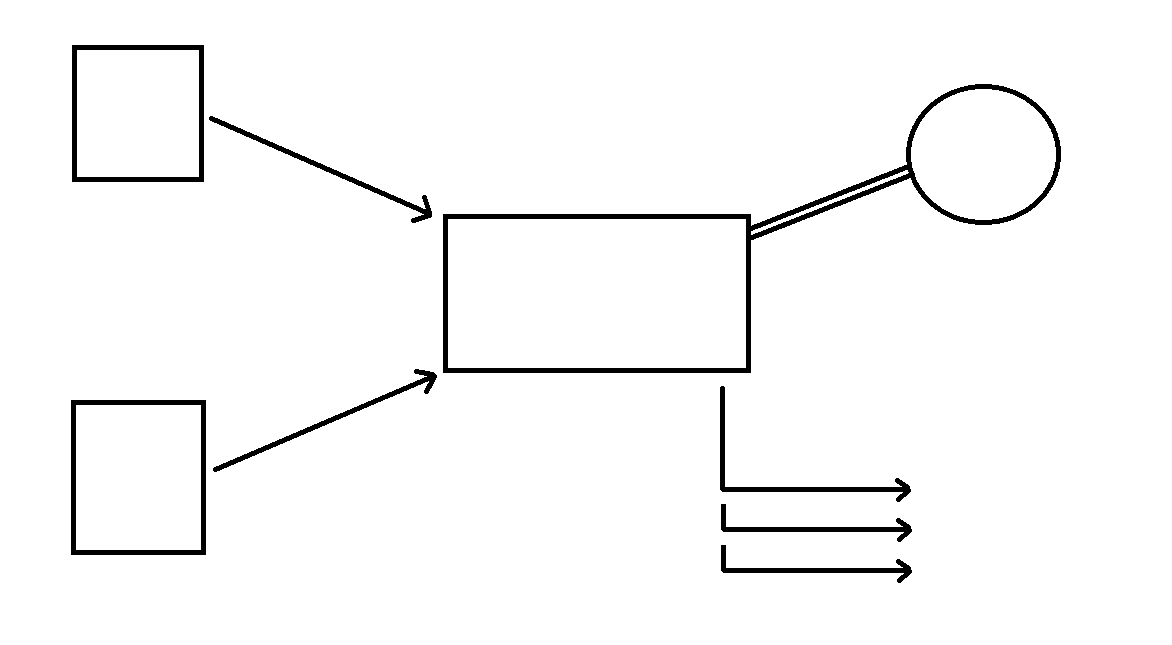
\includegraphics[width=0.8\linewidth]{figs/schema.png}
    \caption{Schéma fonctionnel de la solution existante.}
    \label{fig:schema_existant}
\end{figure}

\subsection{Bilan récapitulatif}
\label{sec:bilan_recap}
% Voici un exemple de tableau comparatif. Le paquet 'booktabs' est utilisé pour les lignes.
\begin{table}[H]
\centering
\caption{Comparaison des technologies d'analyse de données.}
\label{tab:tech_comparison}
\begin{tabular}{lccc}
\toprule
\textbf{Technologie} & \textbf{Type} & \textbf{Avantages} & \textbf{Inconvénients} \\
\midrule
Solution A & Cloud & Scalabilité, Maintenance réduite & Coût, Dépendance \\
Solution B & On-premise & Contrôle, Sécurité & Coût initial, Maintenance \\
Solution C & Hybride & Flexibilité & Complexité \\
\bottomrule
\end{tabular}
\end{table}

% [Votre texte ici]
%\lipsum[7] 
\section{Analyse des besoins}
\label{chap:analyse_besoins}
% [Votre texte ici]
%\lipsum[1]

\subsection{Besoins fonctionnels}
\label{sec:besoins_fonctionnels}
% Vous pouvez lister les besoins fonctionnels dans un tableau comme ci-dessous.
\begin{table}[H]
    \centering
    \caption{Exigences fonctionnelles}
    \label{tab:besoins_fonctionnels}
    \begin{tabularx}{\textwidth}{c X}
        \toprule
        \textbf{ID} & \textbf{Description} \\
        \midrule
        BF-01 & Le système doit permettre l'importation de données depuis des fichiers CSV. \\
        BF-02 & Le système doit fournir un tableau de bord pour visualiser les indicateurs clés de performance (KPIs). \\
        BF-03 & L'utilisateur doit pouvoir exporter les résultats des analyses au format PDF. \\
        \bottomrule
    \end{tabularx}
\end{table}

\subsubsection{Sous-partie 1}
\label{ssec:besoins_fonc_1}
% [Votre texte ici]
%\lipsum[2]

\subsubsection{Sous-partie 2}
\label{ssec:besoins_fonc_2}
% [Votre texte ici]
%\lipsum[3]

\subsection{Besoins non-fonctionnels}
\label{sec:besoins_non_fonctionnels}
% Exemple avec une note de bas de page\footnote{Les notes de bas de page sont utiles pour des informations complémentaires.}
\lipsum[4]
\begin{table}[H]
    \centering
    \caption{Exigences non-fonctionnelles}
    \label{tab:besoins_non_fonctionnels}
    \begin{tabularx}{\textwidth}{c X}
        \toprule
        \textbf{ID} & \textbf{Description} \\
        \midrule
        BNF-01 & Le système doit répondre à une requête en moins de 2 secondes avec 100 utilisateurs concurrents. \\
        BNF-02 & L'interface utilisateur doit être conforme à la charte graphique d'Atos. \\
        BNF-03 & Les données sensibles doivent être chiffrées au repos et en transit. \\
        \bottomrule
    \end{tabularx}
\end{table}

\subsubsection{Sous-partie 1}
\label{ssec:besoins_non_fonc_1}
% [Votre texte ici]
%\lipsum[5]

\subsubsection{Sous-partie 2}
\label{ssec:besoins_non_fonc_2}
% [Votre texte ici]
%\lipsum[6]

\subsection{Développement}
\label{sec:developpement}
% [Votre texte ici]
%\lipsum[7]
\subsubsection{Tâches}
\label{ssec:taches}
% [Votre texte ici]
%\lipsum[8]

\subsubsection{Tests}
\label{ssec:tests}
% [Votre texte ici]
%\lipsum[9] 
\section{Autre partie}
\label{chap:autre_partie}
% [Votre texte ici]
%\lipsum[1]
\subsection{Partie 1}
\label{sec:autre_partie_1}

\subsubsection{Sous-partie 1}
\label{ssec:autre_partie_1_1}
% Pour citer une source, utilisez la commande \cite{cle_bibtex}.
% Par exemple, les travaux de LeCun et al. ont été fondamentaux dans le domaine du Deep Learning \cite{lecun2015deep}.
Le Deep Learning est un domaine de l'intelligence artificielle qui a connu une croissance exponentielle, comme décrit dans l'ouvrage de référence de Goodfellow et al. \cite{goodfellow2016deep}. 
De nombreux outils open-source, tels que TensorFlow \cite{tensorflow2022}, ont rendu ces technologies accessibles.

\subsubsection{Sous-partie 2}
\label{ssec:autre_partie_1_2}
% [Votre texte ici]
%\lipsum[2]
\paragraph{Sous-sous-partie 1}
\label{sssec:autre_partie_1_2_1}
% [Votre texte ici]
%\lipsum[3]

\paragraph{Sous-sous-partie 2}
\label{sssec:autre_partie_1_2_2}
% [Votre texte ici]
%\lipsum[4]
\subparagraph{Paragraphe 1 (agissant comme titre niveau 5)}
% [Votre texte ici]
%\lipsum[5]

\subparagraph{Paragraphe 2}
% [Votre texte ici]
%\lipsum[6]

\paragraph{Sous-sous-partie 3}
\label{sssec:autre_partie_1_2_3}
% [Votre texte ici]
%\lipsum[7]

\subsection{Partie 2}
\label{sec:autre_partie_2}
% [Votre texte ici]
%\lipsum[8]
\subsubsection{Sous-partie 1}
\label{ssec:autre_partie_2_1}
% [Votre texte ici]
%\lipsum[9]

\subsubsection{Sous-partie 2}
\label{ssec:autre_partie_2_2}
% [Votre texte ici]
%\lipsum[10]

\subsubsection{Sous-partie 3}
\label{ssec:autre_partie_2_3}
% [Votre texte ici]
%\lipsum[11] 
\section{Résultats}
\label{chap:resultats}
% [Votre texte ici]
%\lipsum[1-2]

\subsection{Partie 1}
\label{sec:resultats_partie1}
% [Votre texte ici]
%\lipsum[3]
% Voici un exemple de graphique généré avec le paquet PGFPlots.
% C'est très utile pour les graphiques de performance ou les visualisations de données.
\begin{figure}[H]
    \centering
    \begin{tikzpicture}
        \begin{axis}[
            title={Performance du Modèle en fonction des Époques},
            xlabel={Nombre d'époques},
            ylabel={Précision (Accuracy)},
            xmin=0, xmax=100,
            ymin=0.6, ymax=1,
            xtick={0,20,40,60,80,100},
            ytick={0.6,0.7,0.8,0.9,1.0},
            legend pos=outer north east,
            grid=major,
            ]
            \addplot[color=blue, mark=square,]
            coordinates {
                (0,0.65)(20,0.82)(40,0.88)(60,0.91)(80,0.93)(100,0.94)
            };
            \addlegendentry{Précision sur l'ensemble de validation}
        \end{axis}
    \end{tikzpicture}
    \caption{Courbe d'apprentissage du modèle d'IA.}
    \label{fig:learning_curve}
\end{figure}

\subsubsection{Sous-partie 1}
\label{ssec:resultats_p1_s1}
% [Votre texte ici]
%\lipsum[4]

\subsubsection{Sous-partie 2}
\label{ssec:resultats_p1_s2}
% [Votre texte ici]
%\lipsum[5]

\subsubsection{Sous-partie 3}
\label{ssec:resultats_p1_s3}
% [Votre texte ici]
%\lipsum[6]

\subsection{Partie 2}
\label{sec:resultats_partie2}
% [Votre texte ici]
%\lipsum[7]
% Voici un autre exemple d'image, cette fois pour montrer un résultat final.
% La taille est ici fixée à 50% de la largeur du texte.
\begin{figure}[H]
    \centering
    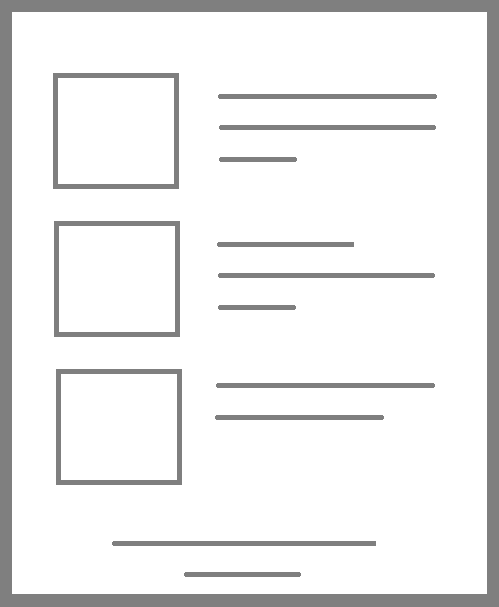
\includegraphics[width=0.5\linewidth]{figs/rendu.png}
    \caption{Exemple de rendu visuel généré par la solution.}
    \label{fig:rendu_final}
\end{figure} 
\section{Bilan}
\label{chap:bilan}
% Contenu du bilan. Vous pouvez discuter des résultats obtenus, 
% des difficultés rencontrées, des compétences acquises et des perspectives futures. 
\appendix

\section{Annexe 1}
\label{sec:annexe1}

\subsection{Partie 1}
\label{ssec:annexe1_partie1}
%Contenu
\subsubsection{Sous-partie 1}
\label{sssec:annexe1_partie1_sous1}
%Contenu
\subsubsection{Sous-partie 2}
\label{sssec:annexe1_partie1_sous2}
%Contenu
\subsubsection{Sous-partie 3}
\label{sssec:annexe1_partie1_sous3}
%Contenu

\subsection{Partie 2}
\label{ssec:annexe1_partie2}
%Contenu
\subsubsection{Sous-partie 1}
\label{sssec:annexe1_partie2_sous1}
%Contenu
\subsubsection{Sous-partie 2}
\label{sssec:annexe1_partie2_sous2}
%Contenu
\subsubsection{Sous-partie 3}
\label{sssec:annexe1_partie2_sous3}
%Contenu

\section{Annexe 2}
\label{sec:annexe2}
%Contenu
\subsection{Prérequis}
\label{ssec:annexe2_prerequis}
%Contenu
\subsection{Partie 1}
\label{ssec:annexe2_partie1}
%Contenu
\subsubsection{Sous-partie 1}
\label{sssec:annexe2_partie1_sous1}
%Contenu
\subsubsection{Sous-partie 2}
\label{sssec:annexe2_partie1_sous2}
%Contenu
\subsection{Partie 2}
\label{ssec:annexe2_partie2}
%Contenu
\subsection{Partie 3}
\label{ssec:annexe2_partie3}
%Contenu 


\newpage
\addcontentsline{toc}{section}{Bibliographie}
\printbibliography[title={References}]

\end{document}